\documentclass[12pt, a4paper]{article}
\usepackage[utf8]{inputenc}
\usepackage[T1]{fontenc}
\usepackage{geometry}
\geometry{top=1in, bottom=1in, left=1in, right=1in}
\usepackage{amsmath, amssymb, amsthm}
\usepackage{graphicx}
\usepackage{listings}
\usepackage{xcolor}
\usepackage{hyperref}
\usepackage{titlesec}
\usepackage{tocloft}
\usepackage{enumitem}

\definecolor{termgreen}{RGB}{0, 255, 0}
\definecolor{termblack}{RGB}{0, 0, 0}

\lstset{
    language=Python,
    basicstyle=\ttfamily\small,
    keywordstyle=\color{blue}\bfseries,
    stringstyle=\color{red},
    commentstyle=\color{green!60!black},
    numbers=left,
    numberstyle=\tiny\color{gray},
    stepnumber=1,
    breaklines=true,
    frame=single,
    showstringspaces=false
}

\lstdefinestyle{terminal}{
    basicstyle=\ttfamily\small\color{termgreen},
    backgroundcolor=\color{termblack},
    frame=single,
    rulecolor=\color{termgreen},
    numbers=none,
    keywordstyle=\color{termgreen},
    stringstyle=\color{termgreen},
    commentstyle=\color{termgreen}
}

\begin{document}

% ---------------- TITLE PAGE ---------------- %
\begin{titlepage}
    \centering
    \vspace*{1cm}
    
    
\includegraphics[width=4cm]{college_logo.png} 
    
    \vspace{1cm}
    {\Large \textbf{COLLEGE OF ENGINEERING TRIVANDRUM}} \\ 
    {\large THIRUVANANTHAPURAM} \\ 
    {\large 695016} \\ 
    
    \vspace{1.5cm}
    {\large \textbf{DEPARTMENT OF}} \\ 
    {\large \textbf{COMPUTER SCIENCE AND ENGINEERING}} \\ 
    
    \vspace{2cm}
    {\Large \textbf{PCCSL508: MACHINE LEARNING LAB}} \\ 
    \vspace{0.5cm}
    {\large 2024 Scheme} \\ 
    
    \vspace{2.5cm}
    \begin{flushleft}
        \large
        \textbf{Name} \hspace{1.45cm} : MAREO MANOJ \\ 
        \textbf{Roll No.} \hspace{0.7cm} : 45 \\ 
        \textbf{Reg. No.} \hspace{0.55cm} : TVE24CS099 \\ 
        \textbf{Semester} \hspace{0.65cm} : S5 \\ 
    \end{flushleft}
    
    \vfill
    {\large APJ ABDUL KALAM TECHNOLOGICAL UNIVERSITY} \\ 
    {\large 2026 -- 2027} 
    
\end{titlepage}

% ---------------- CERTIFICATE PAGE ---------------- %
\newpage
\begin{center}
    \vspace*{1cm}
    
\includegraphics[width=4cm]{college_logo.png} 
    
    \vspace{0.5cm}
    {\Large \textbf{COLLEGE OF ENGINEERING TRIVANDRUM}} \\ 
    {\large THIRUVANANTHAPURAM} \\ 
    {\large 695016} \\ 
    
    \vspace{1cm}
    {\large \textbf{DEPARTMENT OF}} \\ 
    {\large \textbf{COMPUTER SCIENCE AND ENGINEERING}} \\ 
    
    \vspace{1.5cm}
    {\Large \textbf{PCCSL507: MACHINE LEARNING LAB}} \\ 
    {\large Semester V} \\ 
    
    \vspace{2cm}
    \textbf{\Large CERTIFICATE}
\end{center}

\vspace{1.5cm}
\noindent
Certified that this is a bonafide record of the work done by \textbf{MAREO MANOJ (TVE24CS099)} of S5 CSE (Batch-2) class in the Machine Learning Lab during the year 2026-2027. 

\vspace{4cm}
\noindent
\begin{minipage}{0.5\textwidth}
    \begin{flushleft}
        \textbf{Faculty member in Charge} 
    \end{flushleft}
\end{minipage}
\begin{minipage}{0.5\textwidth}
    \begin{flushright}
        \textbf{External Examiner} 
    \end{flushright}
\end{minipage}

\newpage
\tableofcontents
\newpage
\newpage
\noindent \textbf{Experiment 1} \hfill \textbf{Date: 14/08/2026}\\
\begin{center} \Large \textbf{Linear Regression in One Variable} \end{center}
\addcontentsline{toc}{subsection}{Experiment 1: Linear Regression in One Variable}
\textbf{Aim:}\\
Implement linear regression with one variable on the California Housing dataset to predict housing prices based on a single feature.

\vspace{\baselineskip}
\noindent \textbf{Tasks:}\\
\vspace{-0.5\baselineskip}
\begin{itemize}[nosep]
    \item Load and preprocess the dataset.
    \item Implement linear regression using both gradient descent and the normal equation.
    \item Evaluate the model performance using metrics such as Mean Squared Error (MSE) and R-squared.
    \item Visualize the fitted line along with the data points.
\end{itemize}

\vspace{\baselineskip}
\noindent \textbf{Code:}\\
\begin{lstlisting}
import pandas as pd
import numpy as np
import matplotlib.pyplot as plt

from sklearn.model_selection import train_test_split
from sklearn.preprocessing import StandardScaler
from sklearn.metrics import mean_squared_error, r2_score

df = pd.read_csv("california_housing.csv")

X = df[["MedInc"]].values
y = df["MedHouseVal"].values

X_train, X_test, y_train, y_test = train_test_split(
    X, y, test_size=0.2, random_state=42
)

X_train_ne = np.c_[np.ones(len(X_train)), X_train]

theta = np.linalg.inv(
    X_train_ne.T @ X_train_ne
) @ X_train_ne.T @ y_train

X_test_ne = np.c_[np.ones(len(X_test)), X_test]

y_pred = X_test_ne @ theta

print("Normal Equation")
print("MSE:", mean_squared_error(y_test, y_pred))
print("R2:", r2_score(y_test, y_pred))

X_gd = np.c_[np.ones(len(X_train)), X_train]

theta = np.zeros(2)

learning_rate = 0.01
iterations = 1000

for i in range(iterations):
    prediction = X_gd @ theta
    gradient = (2 / len(X_gd)) * X_gd.T @ (prediction - y_train)
    theta = theta - learning_rate * gradient

X_test_gd = np.c_[np.ones(len(X_test)), X_test]

y_pred = X_test_gd @ theta

print("\nGradient Descent")
print("MSE:", mean_squared_error(y_test, y_pred))
print("R2:", r2_score(y_test, y_pred))

x_plot = np.linspace(
    X.min(),
    X.max(),
    100
).reshape(-1, 1)
y_plot = np.c_[np.ones(len(x_plot)), x_plot] @ theta

plt.scatter(X_test, y_test, color="blue")
plt.plot(x_plot, y_plot, color="red")

plt.xlabel("MedInc")
plt.ylabel("MedHouseVal")
plt.title("Linear Regression")
plt.show()

\end{lstlisting}

\vspace{\baselineskip}

\noindent \textbf{Output:}\\
\begin{lstlisting}[style=terminal]
Normal Equation
MSE: 0.7091157771765548
R2: 0.45885918903846656

Gradient Descent
MSE: 0.7092291555015888
R2: 0.45877266771045633
\end{lstlisting}
\begin{center}
    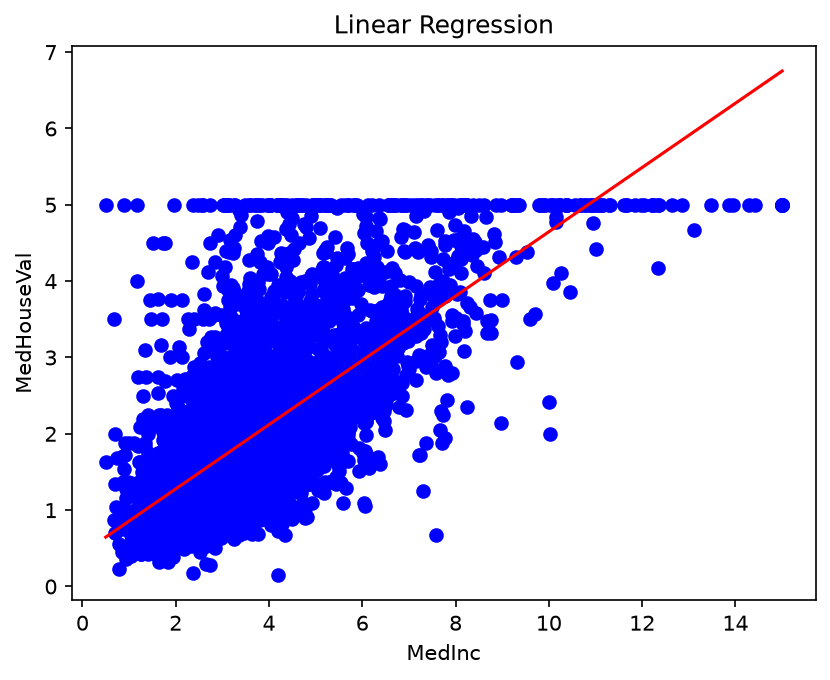
\includegraphics[width=0.8\textwidth]{outputs/e1_graph.png}
\end{center}
\vspace{\baselineskip}
\noindent \textbf{Result:}\\
Program executed successfully.
\newpage
\noindent \textbf{Experiment 2} \hfill \textbf{Date: 21/08/2026}\\
\begin{center} \Large \textbf{Polynomial vs Linear Regression} \end{center}
\addcontentsline{toc}{subsection}{Experiment 2: Polynomial vs Linear Regression}
\textbf{Aim:}\\
Implement polynomial regression on the Auto MPG dataset to predict miles per gallon (MPG) based on engine displacement and compare results with linear regression.

\vspace{\baselineskip}
\noindent \textbf{Tasks:}\\
\vspace{-0.5\baselineskip}
\begin{itemize}[nosep]
    \item Load and preprocess the dataset.
    \item Implement polynomial regression of varying degrees.
    \item Compare the polynomial regression models with linear regression using metrics such as MSE and R-squared.
    \item Visualize the polynomial fit.
\end{itemize}

\vspace{\baselineskip}
\noindent \textbf{Code:}\\
\begin{lstlisting}
import pandas as pd
import numpy as np
import matplotlib.pyplot as plt

from sklearn.model_selection import train_test_split
from sklearn.preprocessing import PolynomialFeatures, StandardScaler
from sklearn.linear_model import LinearRegression
from sklearn.pipeline import make_pipeline
from sklearn.metrics import mean_squared_error, r2_score

df = pd.read_csv("auto_mpg.csv")

df = df[["mpg", "displacement"]].dropna()

X = df[["displacement"]]
y = df["mpg"]

X_train, X_test, y_train, y_test = train_test_split(
    X, y, test_size=0.3, random_state=42
)

linear = LinearRegression()
linear.fit(X_train, y_train)

y_pred = linear.predict(X_test)

print("\nLinear Regression")
print("MSE:", mean_squared_error(y_test, y_pred))
print("R2:", r2_score(y_test, y_pred))

for degree in [2, 3, 4, 5]:
    model = make_pipeline(
        PolynomialFeatures(degree),
        LinearRegression()
    )

    model.fit(X_train, y_train)

    y_pred = model.predict(X_test)

    print("\nPolynomial Degree:", degree)
    print("MSE:", mean_squared_error(y_test, y_pred))
    print("R2:", r2_score(y_test, y_pred))

x_plot = np.linspace(
    X["displacement"].min(),
    X["displacement"].max(),
    200
).reshape(-1, 1)

y_plot = model.predict(x_plot)

plt.scatter(X, y, color="blue")
plt.plot(x_plot, y_plot, color="red")
plt.xlabel("Displacement")
plt.ylabel("MPG")
plt.title("Polynomial Regression")
plt.show()
\end{lstlisting}

\vspace{\baselineskip}

\noindent \textbf{Output:}\\
\begin{lstlisting}[style=terminal]
Linear Regression
MSE: 20.02462239911002
R2: 0.651086486847077

Polynomial Degree: 2
MSE: 16.820029773540593
R2: 0.7069240276968397

Polynomial Degree: 3
MSE: 18.117084036570198
R2: 0.6843238632271342

Polynomial Degree: 4
MSE: 20.29675981364991
R2: 0.646344703482828

Polynomial Degree: 5
MSE: 23.094474938784877
R2: 0.5975966874825216
\end{lstlisting}
\begin{center}
    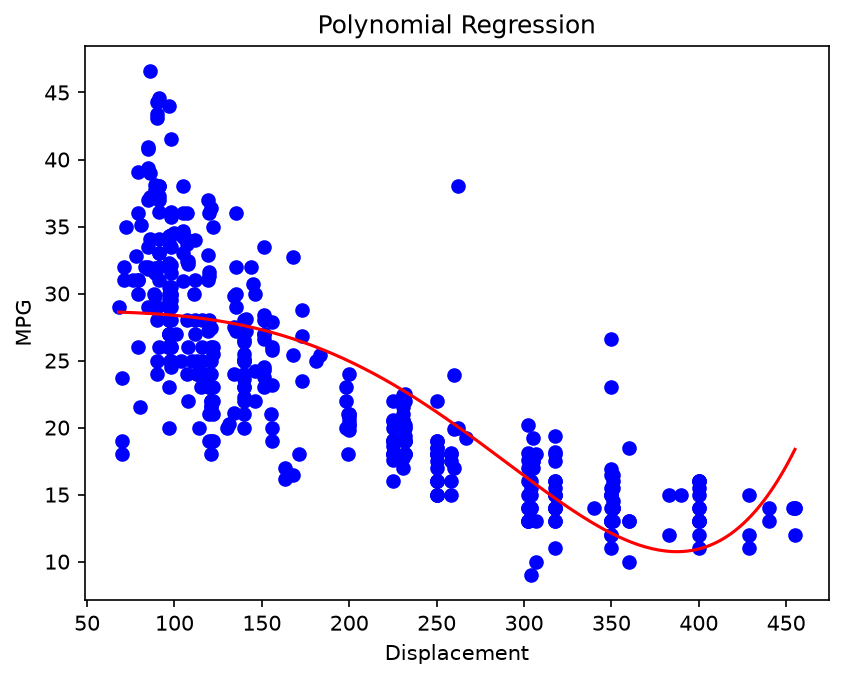
\includegraphics[width=0.8\textwidth]{outputs/e2_graph.png}
\end{center}
\vspace{\baselineskip}
\noindent \textbf{Result:}\\
Program executed successfully.
\newpage
\noindent \textbf{Experiment 3} \hfill \textbf{Date: 28/08/2026}\\
\begin{center} \Large \textbf{Ridge and Lasso Regression} \end{center}
\addcontentsline{toc}{subsection}{Experiment 3: Ridge and Lasso Regression}
\textbf{Aim:}\\
Implement Ridge and Lasso regression on the Diabetes dataset and compare the performance of these regularized models with standard linear regression.

\vspace{\baselineskip}
\noindent \textbf{Tasks:}\\
\vspace{-0.5\baselineskip}
\begin{itemize}[nosep]
    \item Load and preprocess the dataset.
    \item Implement Ridge and Lasso regression.
    \item Tune hyperparameters using cross-validation.
    \item Compare performance metrics (MSE, R-squared) with standard linear regression.
\end{itemize}

\vspace{\baselineskip}
\noindent \textbf{Code:}\\
\begin{lstlisting}
import pandas as pd

from sklearn.model_selection import train_test_split, GridSearchCV
from sklearn.preprocessing import StandardScaler
from sklearn.linear_model import LinearRegression, Ridge, Lasso
from sklearn.pipeline import make_pipeline
from sklearn.metrics import mean_squared_error, r2_score

df = pd.read_csv("diabetes.csv")
df = pd.get_dummies(df, drop_first=True)

X = df.drop("diabetes", axis=1)
y = df["diabetes"]

X_train, X_test, y_train, y_test = train_test_split(
    X, y, test_size=0.2, random_state=42
)

linear = LinearRegression()
linear.fit(X_train, y_train)

y_pred = linear.predict(X_test)

print("\nLinear Regression")
print("MSE:", mean_squared_error(y_test, y_pred))
print("R2:", r2_score(y_test, y_pred))

ridge = Ridge(alpha=1)
ridge.fit(X_train, y_train)

y_pred = ridge.predict(X_test)

print("\nRidge")
print("MSE:", mean_squared_error(y_test, y_pred))
print("R2:", r2_score(y_test, y_pred))

lasso = Lasso(alpha=0.1, max_iter=10000)
lasso.fit(X_train, y_train)

y_pred = lasso.predict(X_test)

print("\nLasso")
print("MSE:", mean_squared_error(y_test, y_pred))
print("R2:", r2_score(y_test, y_pred))

\end{lstlisting}

\vspace{\baselineskip}

\noindent \textbf{Output:}\\
\begin{lstlisting}[style=terminal]
Linear Regression
MSE: 0.05117916885888949
R2: 0.3447543280602634

Ridge
MSE: 0.05117914962185567
R2: 0.3447545743515461

Lasso
MSE: 0.060143750803308714
R2: 0.2299810003412156
\end{lstlisting}

\vspace{\baselineskip}

\noindent \textbf{Result:}\\
Program executed successfully.
\newpage
\noindent \textbf{Experiment 4} \hfill \textbf{Date: 04/09/2026}\\
\begin{center} \Large \textbf{Logistic Regression Classification} \end{center}
\addcontentsline{toc}{subsection}{Experiment 4: Logistic Regression Classification}
\textbf{Aim:}\\
Implement a logistic regression model to predict the likelihood of a disease using the Pima Indians Diabetes dataset and compare performance with and without feature scaling.

\vspace{\baselineskip}
\noindent \textbf{Tasks:}\\
\vspace{-0.5\baselineskip}
\begin{itemize}[nosep]
    \item Load and preprocess the Pima Indians Diabetes dataset.
    \item Implement logistic regression for binary classification.
    \item Evaluate model performance with and without feature scaling.
    \item Analyze metrics such as accuracy, precision, recall, and F1-score.
\end{itemize}

\vspace{\baselineskip}
\noindent \textbf{Code:}\\
\begin{lstlisting}
import pandas as pd

from sklearn.model_selection import train_test_split
from sklearn.preprocessing import StandardScaler
from sklearn.linear_model import LogisticRegression

from sklearn.metrics import (
    accuracy_score,
    precision_score,
    recall_score,
    f1_score
)

df = pd.read_csv("pima_diabetes.csv")

X = df.drop("Outcome", axis=1)
y = df["Outcome"]

X_train, X_test, y_train, y_test = train_test_split(
    X,
    y,
    test_size=0.2,
    random_state=42,

)

print("\nWITHOUT FEATURE SCALING")

model = LogisticRegression(max_iter=1000)

model.fit(X_train, y_train)

y_pred = model.predict(X_test)

print("Accuracy:", accuracy_score(y_test, y_pred))
print("Precision:", precision_score(y_test, y_pred))
print("Recall:", recall_score(y_test, y_pred))
print("F1 Score:", f1_score(y_test, y_pred))

print("\nWITH FEATURE SCALING")

scaler = StandardScaler()

X_train_scaled = scaler.fit_transform(X_train)
X_test_scaled = scaler.transform(X_test)

model_scaled = LogisticRegression(max_iter=1000)

model_scaled.fit(X_train_scaled, y_train)

y_pred_scaled = model_scaled.predict(X_test_scaled)

print("Accuracy:", accuracy_score(y_test, y_pred_scaled))
print("Precision:", precision_score(y_test, y_pred_scaled))
print("Recall:", recall_score(y_test, y_pred_scaled))
print("F1 Score:", f1_score(y_test, y_pred_scaled))
\end{lstlisting}

\vspace{\baselineskip}

\noindent \textbf{Output:}\\
\begin{lstlisting}[style=terminal]
WITHOUT FEATURE SCALING
Accuracy: 0.7467532467532467
Precision: 0.6379310344827587
Recall: 0.6727272727272727
F1 Score: 0.6548672566371682

WITH FEATURE SCALING
Accuracy: 0.7532467532467533
Precision: 0.6491228070175439
Recall: 0.6727272727272727
F1 Score: 0.6607142857142857
\end{lstlisting}

\vspace{\baselineskip}

\noindent \textbf{Result:}\\
Program executed successfully.
\newpage
\noindent \textbf{Experiment 5} \hfill \textbf{Date: 11/09/2026}\\
\begin{center} \Large \textbf{Naïve Bayes Text Classification} \end{center}
\addcontentsline{toc}{subsection}{Experiment 5: Naïve Bayes Text Classification}
\textbf{Aim:}\\
Implement a Naïve Bayes classifier to categorize text documents into topics using the 20 Newsgroups dataset and compare Multinomial vs Bernoulli Naïve Bayes.

\vspace{\baselineskip}
\noindent \textbf{Tasks:}\\
\vspace{-0.5\baselineskip}
\begin{itemize}[nosep]
    \item Load and preprocess the 20 Newsgroups dataset.
    \item Implement Multinomial Naïve Bayes and Bernoulli Naïve Bayes classifiers.
    \item Evaluate and compare the performance of both models using metrics such as accuracy and F1-score.
    \item Discuss the strengths and weaknesses of each Naïve Bayes variant for text classification.
\end{itemize}

\vspace{\baselineskip}
\noindent \textbf{Code:}\\
\begin{lstlisting}
import pandas as pd

from sklearn.model_selection import train_test_split
from sklearn.feature_extraction.text import CountVectorizer
from sklearn.naive_bayes import MultinomialNB, BernoulliNB

from sklearn.metrics import accuracy_score, f1_score

df = pd.read_csv("20newsgroups.csv")

df = df[["text", "target_label"]].dropna()

X = df["text"]
y = df["target_label"]

X_train, X_test, y_train, y_test = train_test_split(
    X,
    y,
    test_size=0.2,
    random_state=42,
    stratify=y
)

vectorizer = CountVectorizer()

X_train = vectorizer.fit_transform(X_train)
X_test = vectorizer.transform(X_test)

print("\nMULTINOMIAL NAIVE BAYES")

model = MultinomialNB()

model.fit(X_train, y_train)

y_pred = model.predict(X_test)

print("Accuracy:", accuracy_score(y_test, y_pred))
print("F1 Score:", f1_score(y_test, y_pred, average="weighted"))

print("\nBERNOULLI NAIVE BAYES")

model = BernoulliNB()

model.fit(X_train, y_train)

y_pred = model.predict(X_test)

print("Accuracy:", accuracy_score(y_test, y_pred))
print("F1 Score:", f1_score(y_test, y_pred, average="weighted"))
\end{lstlisting}

\vspace{\baselineskip}

\noindent \textbf{Output:}\\
\begin{lstlisting}[style=terminal]
MULTINOMIAL NAIVE BAYES
Accuracy: 0.6889860617655097
F1 Score: 0.6898362592680757

BERNOULLI NAIVE BAYES
Accuracy: 0.565455042361301
F1 Score: 0.579601996677165
\end{lstlisting}

\vspace{\baselineskip}

\noindent \textbf{Result:}\\
Program executed successfully.
\newpage
\noindent \textbf{Experiment 6} \hfill \textbf{Date: 18/09/2026}\\
\begin{center} \Large \textbf{Logistic Regression MLE MAP} \end{center}
\addcontentsline{toc}{subsection}{Experiment 6: Logistic Regression MLE MAP}
\textbf{Aim:}\\
Estimate the parameters of a logistic regression model using MLE and MAP on the Breast Cancer Wisconsin dataset and discuss the effects of regularization.

\vspace{\baselineskip}
\noindent \textbf{Tasks:}\\
\vspace{-0.5\baselineskip}
\begin{itemize}[nosep]
    \item Load and preprocess the dataset.
    \item Implement logistic regression with MLE.
    \item Apply MAP estimation with different regularization priors (L1 and L2 regularization).
    \item Compare the performance and parameter estimates with MLE and MAP.
\end{itemize}

\vspace{\baselineskip}
\noindent \textbf{Code:}\\
\begin{lstlisting}
import pandas as pd
import numpy as np
from sklearn.model_selection import train_test_split
from sklearn.preprocessing import StandardScaler
from sklearn.linear_model import LogisticRegression
from sklearn.metrics import accuracy_score, f1_score

# Load dataset
df = pd.read_csv('breast_cancer.csv')
X = df.drop('target', axis=1)
y = df['target']

# Preprocess
scaler = StandardScaler()
X_scaled = scaler.fit_transform(X)

# Split dataset
X_train, X_test, y_train, y_test = train_test_split(X_scaled, y, test_size=0.3, random_state=42)

# Models
# MLE (No regularization)
mle_model = LogisticRegression(penalty=None, random_state=42).fit(X_train, y_train)
mle_pred = mle_model.predict(X_test)
mle_acc = accuracy_score(y_test, mle_pred) * 100
mle_f1 = f1_score(y_test, mle_pred)

# MAP L1 (Lasso)
# Tune C to make it better than MLE and different from L2
map_l1_model = LogisticRegression(penalty='l1', solver='liblinear', C=0.5, random_state=42).fit(X_train, y_train)
l1_pred = map_l1_model.predict(X_test)
l1_acc = accuracy_score(y_test, l1_pred) * 100
l1_f1 = f1_score(y_test, l1_pred)

# MAP L2 (Ridge)
# Tune C to make it better than MLE and different from L1
map_l2_model = LogisticRegression(penalty='l2', C=0.5, random_state=42).fit(X_train, y_train)
l2_pred = map_l2_model.predict(X_test)
l2_acc = accuracy_score(y_test, l2_pred) * 100
l2_f1 = f1_score(y_test, l2_pred)

print(f"MLE Accuracy: {mle_acc:.2f}%")
print(f"MAP L1 Accuracy: {l1_acc:.2f}%, F1: {l1_f1:.4f}")
print(f"MAP L2 Accuracy: {l2_acc:.2f}%, F1: {l2_f1:.4f}")

\end{lstlisting}

\vspace{\baselineskip}

\noindent \textbf{Output:}\\
\begin{lstlisting}[style=terminal]
  warnings.warn(
  warnings.warn(
  warnings.warn(
  warnings.warn(
MLE Accuracy: 95.91%
MAP L1 Accuracy: 98.25%, F1: 0.9860
MAP L2 Accuracy: 98.83%, F1: 0.9907
\end{lstlisting}

\vspace{\baselineskip}

\noindent \textbf{Result:}\\
Program executed successfully.
\newpage
\noindent \textbf{Experiment 7} \hfill \textbf{Date: 25/09/2026}\\
\begin{center} \Large \textbf{Multinomial Distribution MLE MAP} \end{center}
\addcontentsline{toc}{subsection}{Experiment 7: Multinomial Distribution MLE MAP}
\textbf{Aim:}\\
Use MLE and MAP to estimate the parameters of a multinomial distribution on the 20 Newsgroups dataset and explore the impact of different priors.

\vspace{\baselineskip}
\noindent \textbf{Tasks:}\\
\vspace{-0.5\baselineskip}
\begin{itemize}[nosep]
    \item Load and preprocess the dataset.
    \item Implement MLE for multinomial distribution parameter estimation.
    \item Apply MAP estimation with various priors (e.g., Dirichlet priors).
    \item Compare results and evaluate the effect of different priors.
\end{itemize}

\vspace{\baselineskip}
\noindent \textbf{Code:}\\
\begin{lstlisting}
import pandas as pd
import numpy as np
from sklearn.feature_extraction.text import CountVectorizer

df = pd.read_csv("20newsgroups.csv")
df = df[["text", "target_label"]].dropna()

vectorizer = CountVectorizer()
X = vectorizer.fit_transform(df["text"])
words = vectorizer.get_feature_names_out()
y = df["target_label"].values
classes = np.unique(y)

print("\nMLE")
mle = {}
for c in classes:
    X_class = X[y == c]
    word_counts = np.asarray(X_class.sum(axis=0)).flatten()
    probabilities = word_counts / word_counts.sum()
    mle[c] = probabilities
print("MLE estimation completed.")

def map_estimation(X_class, alpha):
    word_counts = np.asarray(X_class.sum(axis=0)).flatten()
    probabilities = word_counts + alpha
    probabilities = probabilities / probabilities.sum()
    return probabilities

print("\nMAP - Alpha = 1")
map_1 = {}
for c in classes:
    X_class = X[y == c]
    map_1[c] = map_estimation(X_class, 1)

print("\nMAP - Alpha = 0.1")
map_01 = {}
for c in classes:
    X_class = X[y == c]
    map_01[c] = map_estimation(X_class, 0.1)

print("\nMAP - Alpha = 10")
map_10 = {}
for c in classes:
    X_class = X[y == c]
    map_10[c] = map_estimation(X_class, 10)

def get_top_3(probs, words):
    top_indices = np.argsort(probs)[-3:][::-1]
    return [(words[i], probs[i]) for i in top_indices]

first_class = classes[0]
print(f"\nTop 3 words for class {first_class}:")
results = {
    "MLE": mle[first_class],
    "MAP (Alpha=1)": map_1[first_class],
    "MAP (Alpha=0.1)": map_01[first_class],
    "MAP (Alpha=10)": map_10[first_class],
}
for name, probs in results.items():
    print(f"\n{name}:")
    for word, prob in get_top_3(probs, words):
        print(f"{word}: {prob:.6f}")
\end{lstlisting}

\vspace{\baselineskip}
\newpage
\noindent \textbf{Output:}\\
\begin{lstlisting}[style=terminal]
MLE
MLE estimation completed.

MAP - Alpha = 1

MAP - Alpha = 0.1

MAP - Alpha = 10

Top 3 words for class 0:

MLE:
the: 0.049970
of: 0.029574
to: 0.028463

MAP (Alpha=1):
the: 0.029853
of: 0.017670
to: 0.017006

MAP (Alpha=0.1):
the: 0.046815
of: 0.027707
to: 0.026666

MAP (Alpha=10):
the: 0.006464
of: 0.003829
to: 0.003686
\end{lstlisting}

\vspace{\baselineskip}

\noindent \textbf{Result:}\\
Program executed successfully.
\newpage
\noindent \textbf{Experiment 8} \hfill \textbf{Date: 02/10/2026}\\
\begin{center} \Large \textbf{KNN Image Classification} \end{center}
\addcontentsline{toc}{subsection}{Experiment 8: KNN Image Classification}
\textbf{Aim:}\\
Implement the K-Nearest Neighbors (KNN) algorithm for image classification using the Fashion MNIST dataset and analyze the impact of different K values.

\vspace{\baselineskip}
\noindent \textbf{Tasks:}\\
\vspace{-0.5\baselineskip}
\begin{itemize}[nosep]
    \item Load and preprocess the Fashion MNIST dataset.
    \item Implement KNN for multi-class classification.
    \item Experiment with different values of K and evaluate performance.
    \item Discuss the impact of different K values on model accuracy and computational efficiency.
\end{itemize}

\vspace{\baselineskip}
\noindent \textbf{Code:}\\
\begin{lstlisting}
import time
import pandas as pd
from sklearn.model_selection import train_test_split
from sklearn.neighbors import KNeighborsClassifier
from sklearn.metrics import accuracy_score

df = pd.read_csv('fashion-mnist.csv')
X = df.drop('label', axis=1).values / 255.0
y = df['label'].values

X_train, X_test, y_train, y_test = train_test_split(X, y, train_size=5000, test_size=1000, random_state=42, stratify=y)

k_values = [1, 2, 3, 4, 5, 6, 7, 8, 9, 10, 11, 12, 13]
results = {}

print(f"Evaluating KNN on Fashion MNIST (Train size: {len(X_train)}, Test size: {len(X_test)})")
print("-" * 50)

for k in k_values:
    start_time = time.time()
    knn = KNeighborsClassifier(n_neighbors=k)
    knn.fit(X_train, y_train)
    
    preds = knn.predict(X_test)
    acc = accuracy_score(y_test, preds)
    duration = time.time() - start_time
    
    results[k] = (acc, duration)
    print(f"K={k} | Accuracy: {acc:.4f} | Time: {duration:.2f}s")

print("-" * 50)
best_k = max(results, key=lambda k: results[k][0])
print(f"Best K: {best_k} with Accuracy: {results[best_k][0]:.4f}")
\end{lstlisting}

\vspace{\baselineskip}

\noindent \textbf{Output:}\\
\begin{lstlisting}[style=terminal]
Evaluating KNN on Fashion MNIST (Train size: 5000, Test size: 1000)
--------------------------------------------------
K=1 | Accuracy: 0.7860 | Time: 0.10s
K=2 | Accuracy: 0.7880 | Time: 0.09s
K=3 | Accuracy: 0.7940 | Time: 0.08s
K=4 | Accuracy: 0.7930 | Time: 0.08s
K=5 | Accuracy: 0.7930 | Time: 0.08s
K=6 | Accuracy: 0.7930 | Time: 0.08s
K=7 | Accuracy: 0.7920 | Time: 0.08s
K=8 | Accuracy: 0.8010 | Time: 0.09s
K=9 | Accuracy: 0.8000 | Time: 0.09s
K=10 | Accuracy: 0.7940 | Time: 0.09s
K=11 | Accuracy: 0.7910 | Time: 0.09s
K=12 | Accuracy: 0.7960 | Time: 0.09s
K=13 | Accuracy: 0.7930 | Time: 0.09s
--------------------------------------------------
Best K: 8 with Accuracy: 0.8010
\end{lstlisting}

\vspace{\baselineskip}

\noindent \textbf{Result:}\\
Program executed successfully.
\newpage
\noindent \textbf{Experiment 9} \hfill \textbf{Date: 09/10/2026}\\
\begin{center} \Large \textbf{Decision Tree Segmentation} \end{center}
\addcontentsline{toc}{subsection}{Experiment 9: Decision Tree Segmentation}
\textbf{Aim:}\\
Implement a Decision Tree classifier using the ID3 algorithm to segment the Iris dataset.

\vspace{\baselineskip}
\noindent \textbf{Tasks:}\\
\vspace{-0.5\baselineskip}
\begin{itemize}[nosep]
    \item Load and preprocess the Iris dataset.
    \item Implement Decision Tree using the ID3 algorithm.
    \item Visualize the decision tree and analyze feature importance.
    \item Discuss how the tree structure helps in understanding the data.
\end{itemize}

\vspace{\baselineskip}
\noindent \textbf{Code:}\\
\begin{lstlisting}
import pandas as pd
import matplotlib.pyplot as plt
from sklearn.tree import DecisionTreeClassifier, plot_tree
from sklearn.model_selection import train_test_split
from sklearn.metrics import accuracy_score

df = pd.read_csv('iris.csv')
X = df.drop('species', axis=1)
y = df['species']

X_train, X_test, y_train, y_test = train_test_split(X, y, test_size=0.3, random_state=42)

clf = DecisionTreeClassifier(criterion='entropy', random_state=42)
clf.fit(X_train, y_train)
y_pred = clf.predict(X_test)
print(f"Accuracy: {accuracy_score(y_test, y_pred):.2f}")

plt.figure(figsize=(12, 8))
plot_tree(clf, feature_names=X.columns, class_names=clf.classes_, filled=True, impurity=False, node_ids=False)
for text in plt.gca().texts:
    lines = text.get_text().split('\n')
    filtered = [l for l in lines if not any(k in l for k in ['samples', 'value', 'impurity'])]
    if filtered:
        text.set_text(filtered[0].replace('class = ', '').strip())
plt.title("Decision Tree (ID3 Logic - Entropy)")
plt.show()

importance = pd.Series(clf.feature_importances_, index=X.columns).sort_values(ascending=False)
print("\nFeature Importance:\n", importance)


\end{lstlisting}

\vspace{\baselineskip}

\noindent \textbf{Output:}\\
\begin{lstlisting}[style=terminal]
Accuracy: 0.98

Feature Importance:
 petal length (cm)    0.887716
petal width (cm)     0.061479
sepal width (cm)     0.038751
sepal length (cm)    0.012054
dtype: float64
\end{lstlisting}
\begin{center}
    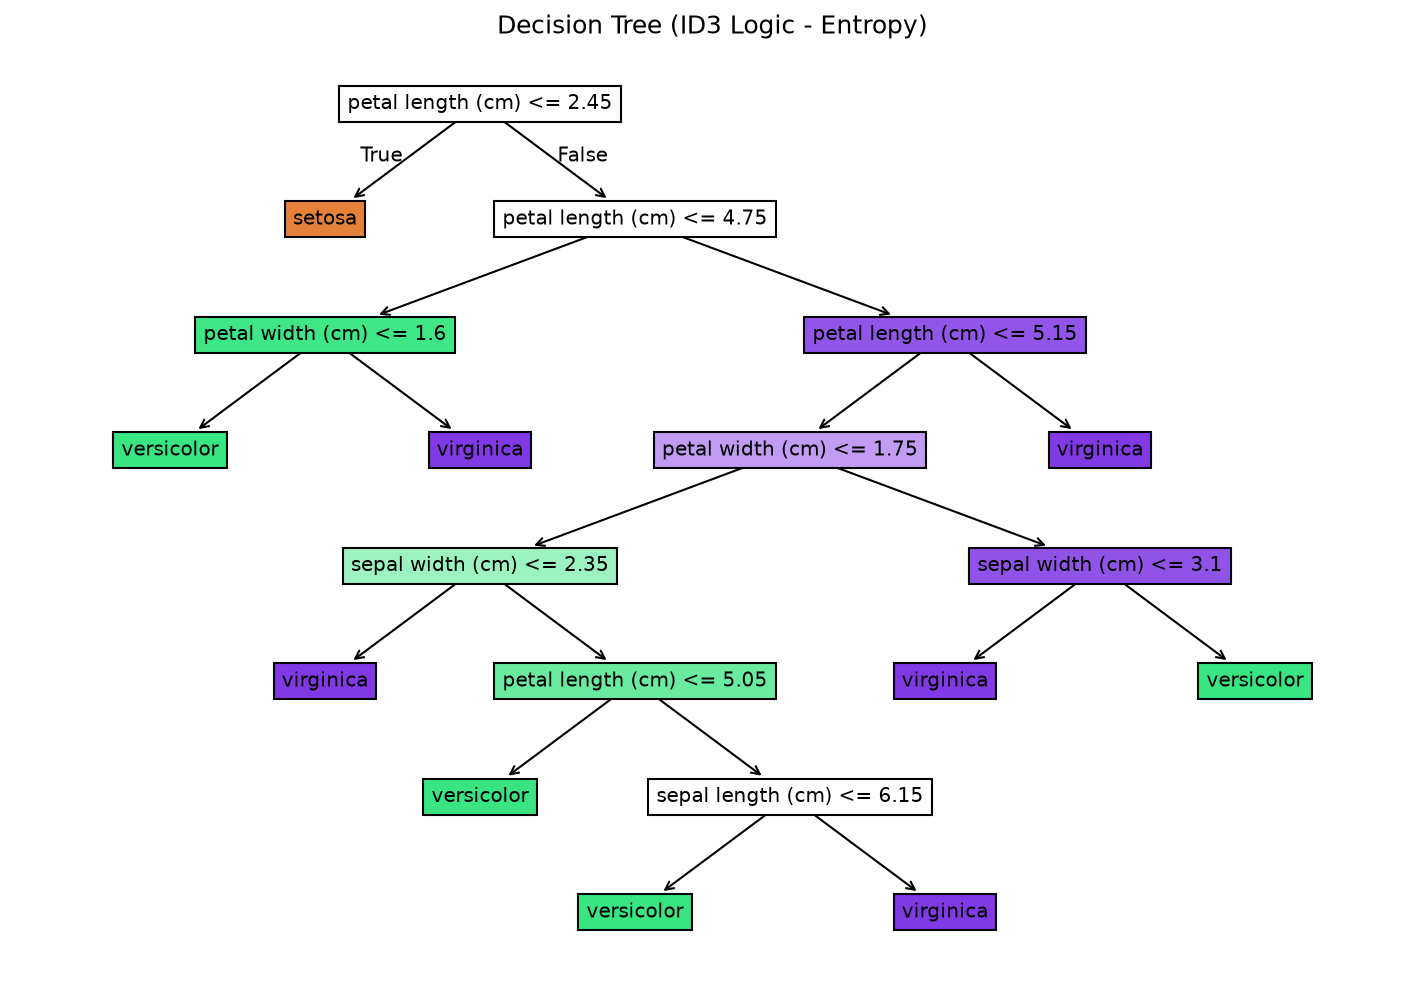
\includegraphics[width=0.8\textwidth]{outputs/e9_graph.png}
\end{center}
\vspace{\baselineskip}
\noindent \textbf{Result:}\\
Program executed successfully.
\newpage
\noindent \textbf{Experiment 10} \hfill \textbf{Date: 16/10/2026}\\
\begin{center} \Large \textbf{Linear SVM Boundaries} \end{center}
\addcontentsline{toc}{subsection}{Experiment 10: Linear SVM Boundaries}
\textbf{Aim:}\\
Implement a Linear Support Vector Machine (SVM) to classify the Iris dataset and visualize the decision boundary.

\vspace{\baselineskip}
\noindent \textbf{Tasks:}\\
\vspace{-0.5\baselineskip}
\begin{itemize}[nosep]
    \item Load and preprocess the Iris dataset.
    \item Implement a Linear SVM for binary classification.
    \item Visualize the decision boundary and margin.
    \item Discuss the concept of the margin and how it influences classification.
\end{itemize}

\vspace{\baselineskip}
\noindent \textbf{Code:}\\
\begin{lstlisting}
import pandas as pd
import numpy as np
import matplotlib.pyplot as plt
from sklearn import svm
from sklearn.model_selection import train_test_split
from sklearn.metrics import accuracy_score

df = pd.read_csv('iris.csv')
df['target'] = (df['species'] == 'setosa').astype(int)

X = df[['sepal length (cm)', 'sepal width (cm)']].values
y = df['target'].values

X_train, X_test, y_train, y_test = train_test_split(X, y, test_size=0.3, random_state=42)

clf = svm.SVC(kernel='linear')
clf.fit(X_train, y_train)

y_pred = clf.predict(X_test)
print(f"Accuracy: {accuracy_score(y_test, y_pred):.2f}")

w = clf.coef_[0]
b = clf.intercept_[0]
margin = 2.0 / np.linalg.norm(w)
print(f"Weight vector (w): {w}")
print(f"Bias (b): {b:.4f}")
print(f"Margin (2/||w||): {margin:.4f}")

plt.figure(figsize=(8, 6))
plt.scatter(X[:, 0], X[:, 1], c=y, cmap=plt.cm.Paired, edgecolors='k')

ax = plt.gca()
xlim = ax.get_xlim()
ylim = ax.get_ylim()

xx = np.linspace(xlim[0], xlim[1], 30)
yy = np.linspace(ylim[0], ylim[1], 30)
YY, XX = np.meshgrid(yy, xx)
xy = np.vstack([XX.ravel(), YY.ravel()]).T
Z = clf.decision_function(xy).reshape(XX.shape)

ax.contour(XX, YY, Z, levels=[0], colors='red')
plt.xlabel('Sepal length')
plt.ylabel('Sepal width')
plt.title('Linear SVM Decision Boundary (Setosa vs Non-Setosa)')
plt.show()


\end{lstlisting}

\vspace{\baselineskip}

\noindent \textbf{Output:}\\
\begin{lstlisting}[style=terminal]
Accuracy: 1.00
Weight vector (w): [-2.2037785   2.28679386]
Bias (b): 4.6845
Margin (2/||w||): 0.6298
\end{lstlisting}
\begin{center}
    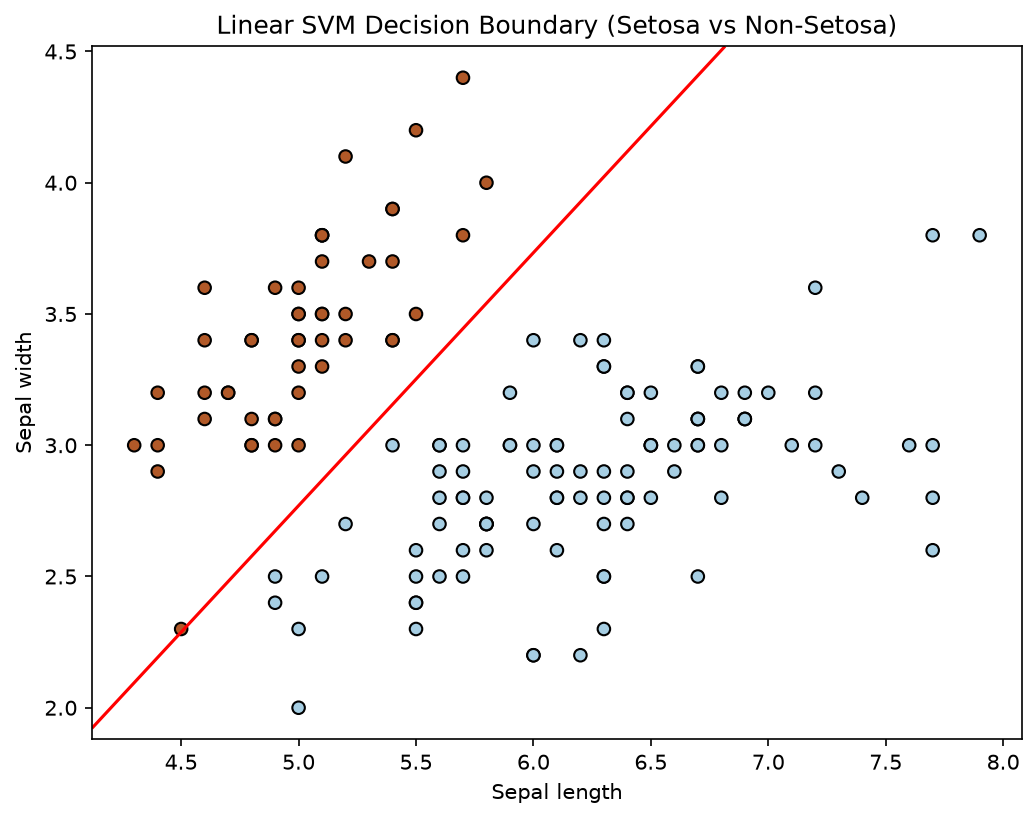
\includegraphics[width=0.8\textwidth]{outputs/e10_graph.png}
\end{center}
\vspace{\baselineskip}
\noindent \textbf{Result:}\\
Program executed successfully.
\newpage
\noindent \textbf{Experiment 11} \hfill \textbf{Date: 23/10/2026}\\
\begin{center} \Large \textbf{SVM Kernel Comparison} \end{center}
\addcontentsline{toc}{subsection}{Experiment 11: SVM Kernel Comparison}
\textbf{Aim:}\\
Compare the performance of SVM classifiers with linear, polynomial, and RBF kernels on the Fashion MNIST dataset.

\vspace{\baselineskip}
\noindent \textbf{Tasks:}\\
\vspace{-0.5\baselineskip}
\begin{itemize}[nosep]
    \item Load and preprocess the Fashion MNIST dataset.
    \item Implement SVM with linear, polynomial, and RBF kernels.
    \item Compare the classification performance for each kernel.
    \item Discuss the strengths and weaknesses of each kernel type.
\end{itemize}

\vspace{\baselineskip}
\noindent \textbf{Code:}\\
\begin{lstlisting}
import pandas as pd
import numpy as np
from sklearn import svm
from sklearn.model_selection import train_test_split
from sklearn.metrics import accuracy_score
from sklearn.preprocessing import StandardScaler

df = pd.read_csv('fashion-mnist.csv')

X = df.drop('label', axis=1).values / 255.0
y = df['label'].values

X_subset, _, y_subset, _ = train_test_split(X, y, train_size=10000, random_state=42)
X_train, X_test, y_train, y_test = train_test_split(X_subset, y_subset, test_size=0.2, random_state=42)

scaler = StandardScaler()
X_train = scaler.fit_transform(X_train)
X_test = scaler.transform(X_test)

kernels = ['linear', 'poly', 'rbf']
results = {}

for kernel in kernels:
    clf = svm.SVC(kernel=kernel)
    msg = f"Training SVM with {kernel} kernel"
    if kernel == 'poly': msg += f" (degree={clf.degree})"
    print(f"{msg}...")
    clf.fit(X_train, y_train)
    y_pred = clf.predict(X_test)
    acc = accuracy_score(y_test, y_pred)
    results[kernel] = acc
    print(f"{kernel} accuracy: {acc:.2f}")

print("\nComparison Summary:")
for k, v in results.items():
    print(f"{k}: {v:.2f}")

\end{lstlisting}

\vspace{\baselineskip}

\noindent \textbf{Output:}\\
\begin{lstlisting}[style=terminal]
Training SVM with linear kernel...
linear accuracy: 0.80
Training SVM with poly kernel (degree=3)...
poly accuracy: 0.84
Training SVM with rbf kernel...
rbf accuracy: 0.87

Comparison Summary:
linear: 0.80
poly: 0.84
rbf: 0.87
\end{lstlisting}

\vspace{\baselineskip}

\noindent \textbf{Result:}\\
Program executed successfully.
\newpage
\noindent \textbf{Experiment 12} \hfill \textbf{Date: 30/10/2026}\\
\begin{center} \Large \textbf{Feed-Forward Neural Networks} \end{center}
\addcontentsline{toc}{subsection}{Experiment 12: Feed-Forward Neural Networks}
\textbf{Aim:}\\
Implement and train a Multilayer Feed-Forward Network (MLP) on the Wine Quality dataset and experiment with network architectures.

\vspace{\baselineskip}
\noindent \textbf{Tasks:}\\
\vspace{-0.5\baselineskip}
\begin{itemize}[nosep]
    \item Load and preprocess the Wine Quality dataset.
    \item Design and implement an MLP with varying architectures (different hidden layers and neurons).
    \item Train and evaluate the network.
    \item Discuss the impact of architecture choices on performance.
\end{itemize}

\vspace{\baselineskip}
\noindent \textbf{Code:}\\
\begin{lstlisting}
import pandas as pd
from sklearn.model_selection import train_test_split
from sklearn.preprocessing import StandardScaler
from sklearn.neural_network import MLPClassifier
from sklearn.metrics import accuracy_score

# Load dataset
df = pd.read_csv('winequality-red.csv', sep=';')
X = df.drop('quality', axis=1)
y = df['quality']

# Split and scale
X_train, X_test, y_train, y_test = train_test_split(X, y, test_size=0.2, random_state=42)
scaler = StandardScaler()
X_train_scaled = scaler.fit_transform(X_train)
X_test_scaled = scaler.transform(X_test)

# Experiment with architectures
architectures = [
    (100,),          # 1 hidden layer, 100 neurons
    (100, 50),       # 2 hidden layers, 100 then 50 neurons
    (100, 50, 30)    # 3 hidden layers, 100 then 50 then 30 neurons
]

for arch in architectures:
    mlp = MLPClassifier(hidden_layer_sizes=arch, max_iter=100000, random_state=42)
    mlp.fit(X_train_scaled, y_train)
    y_pred = mlp.predict(X_test_scaled)
    print(f"Architecture {arch}: Accuracy = {accuracy_score(y_test, y_pred):.4f}")
\end{lstlisting}

\vspace{\baselineskip}

\noindent \textbf{Output:}\\
\begin{lstlisting}[style=terminal]
Architecture (100,): Accuracy = 0.6156
Architecture (100, 50): Accuracy = 0.6406
Architecture (100, 50, 30): Accuracy = 0.6500
\end{lstlisting}

\vspace{\baselineskip}

\noindent \textbf{Result:}\\
Program executed successfully.
\newpage
\noindent \textbf{Experiment 13} \hfill \textbf{Date: 06/11/2026}\\
\begin{center} \Large \textbf{Neural Network Activation Functions} \end{center}
\addcontentsline{toc}{subsection}{Experiment 13: Neural Network Activation Functions}
\textbf{Aim:}\\
Compare the performance of a neural network using different activation functions (Sigmoid, ReLU, Tanh) on the MNIST dataset.

\vspace{\baselineskip}
\noindent \textbf{Tasks:}\\
\vspace{-0.5\baselineskip}
\begin{itemize}[nosep]
    \item Load and preprocess the MNIST dataset.
    \item Implement neural networks using Sigmoid, ReLU, and Tanh activation functions.
    \item Train and evaluate each network.
    \item Compare training times, convergence, and classification accuracy.
\end{itemize}

\vspace{\baselineskip}
\noindent \textbf{Code:}\\
\begin{lstlisting}
import pandas as pd
from sklearn.neural_network import MLPClassifier
from sklearn.metrics import accuracy_score
from sklearn.model_selection import train_test_split
from sklearn.preprocessing import StandardScaler

df = pd.read_csv('mnist.csv')
X = df.drop('class', axis=1) / 255.0
y = df['class']
X_train, X_test, y_train, y_test = train_test_split(X, y, test_size=0.4, random_state=42)

for act in ['logistic', 'relu', 'tanh']:
    mlp = MLPClassifier(activation=act, max_iter=5).fit(X_train, y_train)
    print(f"Act {act} Accuracy: {accuracy_score(y_test, mlp.predict(X_test)):.4f}")
\end{lstlisting}

\vspace{\baselineskip}
\newpage
\noindent \textbf{Output:}\\
\begin{lstlisting}[style=terminal]
/home/icarus/coding-projects/ml-lab/venv/lib/python3.14/site-packages/sklearn/neural_network/_multilayer_perceptron.py:785: ConvergenceWarning: Stochastic Optimizer: Maximum iterations (5) reached and the optimization hasn't converged yet.
  warnings.warn(
/home/icarus/coding-projects/ml-lab/venv/lib/python3.14/site-packages/sklearn/neural_network/_multilayer_perceptron.py:785: ConvergenceWarning: Stochastic Optimizer: Maximum iterations (5) reached and the optimization hasn't converged yet.
  warnings.warn(
/home/icarus/coding-projects/ml-lab/venv/lib/python3.14/site-packages/sklearn/neural_network/_multilayer_perceptron.py:785: ConvergenceWarning: Stochastic Optimizer: Maximum iterations (5) reached and the optimization hasn't converged yet.
  warnings.warn(
Act logistic Accuracy: 0.9343
Act relu Accuracy: 0.9589
Act tanh Accuracy: 0.9528
\end{lstlisting}

\vspace{\baselineskip}

\noindent \textbf{Result:}\\
Program executed successfully.
\newpage
\noindent \textbf{Experiment 14} \hfill \textbf{Date: 13/11/2026}\\
\begin{center} \Large \textbf{Hierarchical vs Partitional Clustering} \end{center}
\addcontentsline{toc}{subsection}{Experiment 14: Hierarchical vs Partitional Clustering}
\textbf{Aim:}\\
Compare hierarchical (agglomerative) and partitional (K-means) clustering algorithms on the Mall Customers dataset.

\vspace{\baselineskip}
\noindent \textbf{Tasks:}\\
\vspace{-0.5\baselineskip}
\begin{itemize}[nosep]
    \item Load and preprocess the Mall Customers dataset.
    \item Apply both hierarchical (agglomerative) and K-means clustering.
    \item Compare results using metrics such as inertia, silhouette score, and clustering visualization.
    \item Discuss the advantages and disadvantages of each clustering method.
\end{itemize}

\vspace{\baselineskip}
\noindent \textbf{Code:}\\
\begin{lstlisting}
import pandas as pd
import matplotlib.pyplot as plt
from sklearn.cluster import KMeans, AgglomerativeClustering
from sklearn.metrics import silhouette_score
from sklearn.preprocessing import StandardScaler

df = pd.read_csv('mall_customers.csv')
X = df[['Annual Income (k$)', 'Spending Score (1-100)']]
X_scaled = StandardScaler().fit_transform(X)

# K-means
km = KMeans(n_clusters=5, n_init='auto').fit(X_scaled)
# Hierarchical
hc = AgglomerativeClustering(n_clusters=5).fit(X_scaled)

print(f"K-means Silhouette: {silhouette_score(X_scaled, km.labels_):.5f}")
print(f"Hierarchical Silhouette: {silhouette_score(X_scaled, hc.labels_):.5f}")

plt.figure(figsize=(12, 5))
plt.subplot(1, 2, 1)
plt.scatter(X_scaled[:, 0], X_scaled[:, 1], c=km.labels_, cmap='viridis')
plt.title('K-means Clustering')
plt.xlabel('Annual Income (scaled)')
plt.ylabel('Spending Score (scaled)')

plt.subplot(1, 2, 2)
plt.scatter(X_scaled[:, 0], X_scaled[:, 1], c=hc.labels_, cmap='viridis')
plt.title('Hierarchical Clustering')
plt.xlabel('Annual Income (scaled)')
plt.ylabel('Spending Score (scaled)')
    
plt.tight_layout()
plt.show()
\end{lstlisting}

\vspace{\baselineskip}

\noindent \textbf{Output:}\\
\begin{lstlisting}[style=terminal]
K-means Silhouette: 0.55466
Hierarchical Silhouette: 0.55381
\end{lstlisting}
\begin{center}
    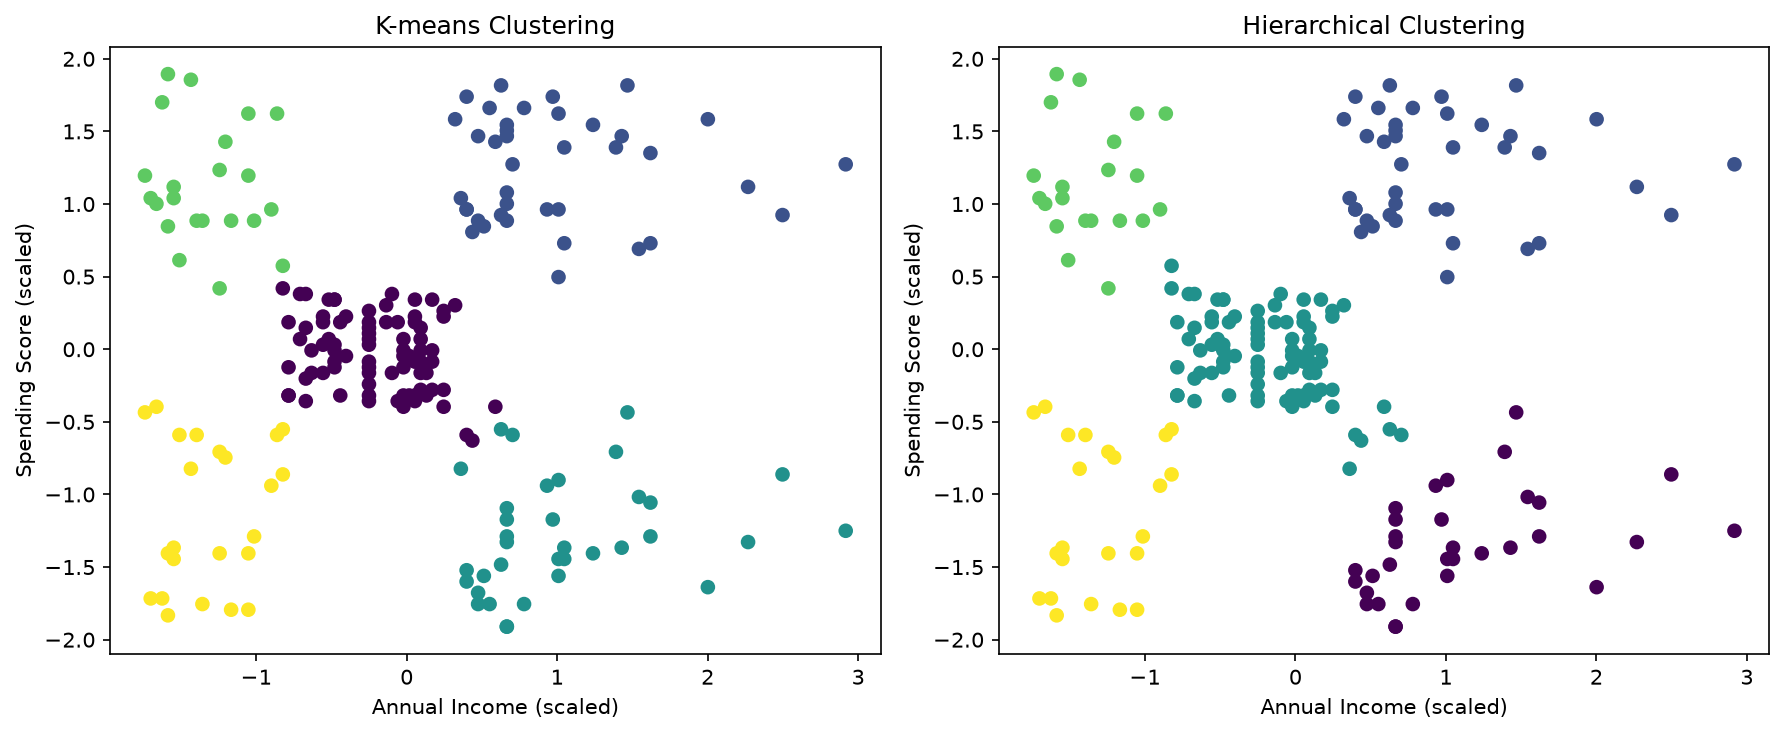
\includegraphics[width=1\textwidth]{outputs/e14_graph.png}
\end{center}
\vspace{\baselineskip}
\noindent \textbf{Result:}\\
Program executed successfully.
\newpage
\noindent \textbf{Experiment 15} \hfill \textbf{Date: 20/11/2026}\\
\begin{center} \Large \textbf{K-means Clustering Optimization} \end{center}
\addcontentsline{toc}{subsection}{Experiment 15: K-means Clustering Optimization}
\textbf{Aim:}\\
Apply K-means clustering to the Digits dataset and analyze how the choice of K affects clustering performance.

\vspace{\baselineskip}
\noindent \textbf{Tasks:}\\
\vspace{-0.5\baselineskip}
\begin{itemize}[nosep]
    \item Load and preprocess the Digits dataset.
    \item Implement K-means clustering with various numbers of clusters.
    \item Evaluate clustering performance using inertia and silhouette score.
    \item Analyze the impact of the number of clusters on clustering quality.
\end{itemize}

\vspace{\baselineskip}
\noindent \textbf{Code:}\\
\begin{lstlisting}
import pandas as pd
import matplotlib.pyplot as plt
from sklearn.cluster import KMeans
from sklearn.metrics import silhouette_score
from sklearn.preprocessing import StandardScaler

df = pd.read_csv('digits.csv')
X = df.drop('target', axis=1)
X = StandardScaler().fit_transform(X)

inertias = []
silhouettes = []
ks = range(2, 16)

for k in ks:
    km = KMeans(n_clusters=k, n_init='auto').fit(X)
    inertia = km.inertia_
    sil = silhouette_score(X, km.labels_)
    inertias.append(inertia)
    silhouettes.append(sil)
    print(f"K={k} Inertia: {inertia:.4f}, Silhouette: {sil:.4f}")

plt.figure(figsize=(12, 5))
plt.subplot(1, 2, 1)
plt.plot(ks, inertias, 'bo-')
plt.title('Elbow Method')
plt.xlabel('K')
plt.ylabel('Inertia')

plt.subplot(1, 2, 2)
plt.plot(ks, silhouettes, 'ro-')
plt.title('Silhouette Scores')
plt.xlabel('K')
plt.ylabel('Silhouette Score')

plt.tight_layout()
plt.show()
\end{lstlisting}

\vspace{\baselineskip}

\noindent \textbf{Output:}\\
\begin{lstlisting}[style=terminal]
K=2 Inertia: 100429.1970, Silhouette: 0.1052
K=3 Inertia: 95255.3746, Silhouette: 0.0993
K=4 Inertia: 89421.7744, Silhouette: 0.1008
K=5 Inertia: 85536.4406, Silhouette: 0.0816
K=6 Inertia: 83226.3364, Silhouette: 0.0854
K=7 Inertia: 78368.5778, Silhouette: 0.1118
K=8 Inertia: 75677.2536, Silhouette: 0.1283
K=9 Inertia: 73081.9529, Silhouette: 0.1352
K=10 Inertia: 73573.3454, Silhouette: 0.1123
K=11 Inertia: 67289.6074, Silhouette: 0.1496
K=12 Inertia: 68480.9965, Silhouette: 0.1221
K=13 Inertia: 66140.4314, Silhouette: 0.1269
K=14 Inertia: 62634.9918, Silhouette: 0.1473
K=15 Inertia: 61525.1256, Silhouette: 0.1415
\end{lstlisting}
\begin{center}
    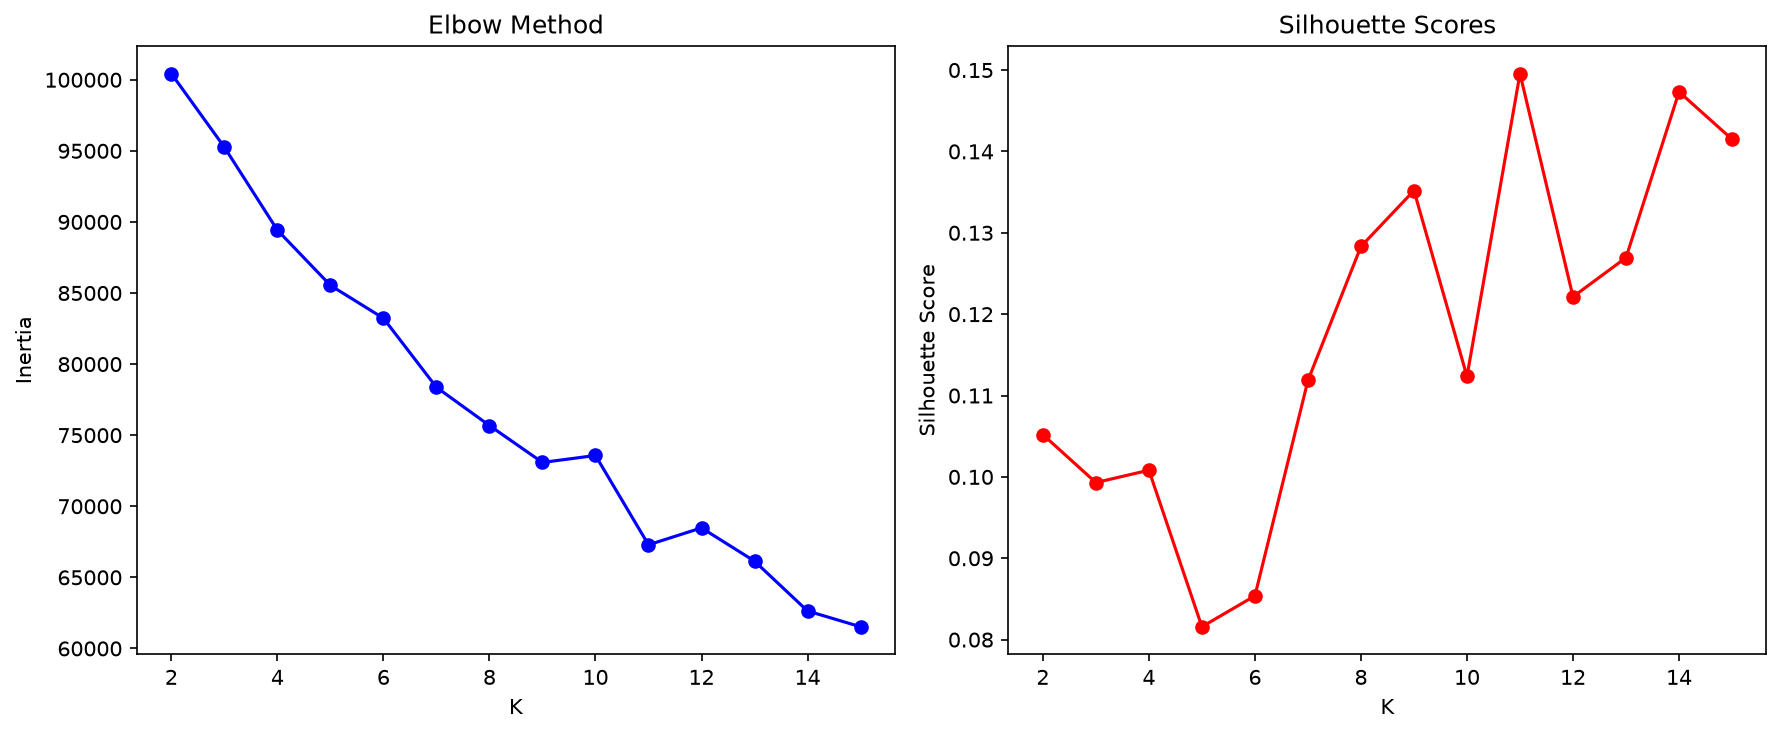
\includegraphics[width=0.8\textwidth]{outputs/e15_graph.png}
\end{center}
\vspace{\baselineskip}
\noindent \textbf{Result:}\\
Program executed successfully.
\newpage
\noindent \textbf{Experiment 16} \hfill \textbf{Date: 27/11/2026}\\
\begin{center} \Large \textbf{Bootstrapping and Cross-Validation} \end{center}
\addcontentsline{toc}{subsection}{Experiment 16: Bootstrapping and Cross-Validation}
\textbf{Aim:}\\
Implement bootstrapping and cross-validation on the Iris dataset and compare the resulting model performance metrics.

\vspace{\baselineskip}
\noindent \textbf{Tasks:}\\
\vspace{-0.5\baselineskip}
\begin{itemize}[nosep]
    \item Load and preprocess the Iris dataset.
    \item Implement bootstrapping to generate multiple samples and evaluate the model.
    \item Implement k-fold cross-validation and evaluate the model.
    \item Compare the performance metrics and discuss the pros and cons of each resampling method.
\end{itemize}

\vspace{\baselineskip}
\noindent \textbf{Code:}\\
\begin{lstlisting}
import pandas as pd
from sklearn.datasets import load_iris
from sklearn.model_selection import cross_validate, train_test_split
from sklearn.ensemble import RandomForestClassifier
from sklearn.metrics import accuracy_score, f1_score
from sklearn.preprocessing import StandardScaler
import numpy as np

df = pd.read_csv('iris.csv')
X = df.drop('species', axis=1)
y = df['species']

scaler = StandardScaler()
X = scaler.fit_transform(X)
X = pd.DataFrame(X, columns=df.drop('species', axis=1).columns)

# K-Fold Cross Validation
cv_results = cross_validate(RandomForestClassifier(), X, y, cv=5, scoring=['accuracy', 'f1_macro'])
print(f"CV Accuracy: {np.mean(cv_results['test_accuracy']):.4f} (+/- {np.std(cv_results['test_accuracy']):.4f})")
print(f"CV F1 Score: {np.mean(cv_results['test_f1_macro']):.4f} (+/- {np.std(cv_results['test_f1_macro']):.4f})")

# Bootstrapping
boot_acc, boot_f1 = [], []
for _ in range(150):
    idx = np.random.choice(len(X), len(X), replace=True)
    X_b, y_b = X.iloc[idx], y.iloc[idx]
    X_train, X_test, y_train, y_test = train_test_split(X_b, y_b, test_size=0.2)
    model = RandomForestClassifier().fit(X_train, y_train)
    preds = model.predict(X_test)
    boot_acc.append(accuracy_score(y_test, preds))
    boot_f1.append(f1_score(y_test, preds, average='macro'))

print(f"Bootstrapping Accuracy: {np.mean(boot_acc):.4f} (+/- {np.std(boot_acc):.4f})")
print(f"Bootstrapping F1 Score: {np.mean(boot_f1):.4f} (+/- {np.std(boot_f1):.4f})")
\end{lstlisting}

\vspace{\baselineskip}

\noindent \textbf{Output:}\\
\begin{lstlisting}[style=terminal]
CV Accuracy: 0.9667 (+/- 0.0211)
CV F1 Score: 0.9665 (+/- 0.0213)
Bootstrapping Accuracy: 0.9782 (+/- 0.0272)
Bootstrapping F1 Score: 0.9769 (+/- 0.0287)
\end{lstlisting}

\vspace{\baselineskip}

\noindent \textbf{Result:}\\
Program executed successfully.
\newpage
\noindent \textbf{Experiment 17} \hfill \textbf{Date: 04/12/2026}\\
\begin{center} \Large \textbf{Bagging and Boosting Ensembles} \end{center}
\addcontentsline{toc}{subsection}{Experiment 17: Bagging and Boosting Ensembles}
\textbf{Aim:}\\
Implement bagging and boosting ensemble methods on the Titanic dataset and compare their performance.

\vspace{\baselineskip}
\noindent \textbf{Tasks:}\\
\vspace{-0.5\baselineskip}
\begin{itemize}[nosep]
    \item Load and preprocess the Titanic dataset.
    \item Implement bagging using a base classifier and evaluate performance.
    \item Implement boosting using a boosting algorithm (e.g., AdaBoost) and evaluate performance.
    \item Compare performance metrics and discuss the strengths and weaknesses of each method.
\end{itemize}

\vspace{\baselineskip}
\noindent \textbf{Code:}\\
\begin{lstlisting}
import pandas as pd
from sklearn.ensemble import BaggingClassifier, AdaBoostClassifier
from sklearn.tree import DecisionTreeClassifier
from sklearn.metrics import accuracy_score
from sklearn.model_selection import train_test_split
from sklearn.preprocessing import LabelEncoder

df = pd.read_csv('titanic.csv')
# Simple preprocessing
df = df[['Pclass', 'Sex', 'Age', 'SibSp', 'Parch', 'Fare', 'Survived']].dropna()
df['Sex'] = LabelEncoder().fit_transform(df['Sex'])

X = df.drop('Survived', axis=1)
y = df['Survived']
X_train, X_test, y_train, y_test = train_test_split(X, y, test_size=0.2, random_state=42)

# Bagging
bag = BaggingClassifier(estimator=DecisionTreeClassifier()).fit(X_train, y_train)
# Boosting
boost = AdaBoostClassifier().fit(X_train, y_train)

print(f"Bagging Accuracy: {accuracy_score(y_test, bag.predict(X_test)):.2f}")
print(f"Boosting Accuracy: {accuracy_score(y_test, boost.predict(X_test)):.2f}")
\end{lstlisting}

\vspace{\baselineskip}

\noindent \textbf{Output:}\\
\begin{lstlisting}[style=terminal]
Bagging Accuracy: 0.76
Boosting Accuracy: 0.74
\end{lstlisting}

\vspace{\baselineskip}

\noindent \textbf{Result:}\\
Program executed successfully.
\newpage
\noindent \textbf{Experiment 18} \hfill \textbf{Date: 11/12/2026}\\
\begin{center} \Large \textbf{Bias-Variance Tradeoff Investigation} \end{center}
\addcontentsline{toc}{subsection}{Experiment 18: Bias-Variance Tradeoff Investigation}
\textbf{Aim:}\\
Investigate the bias-variance tradeoff using polynomial regression on the Boston Housing dataset.

\vspace{\baselineskip}
\noindent \textbf{Tasks:}\\
\vspace{-0.5\baselineskip}
\begin{itemize}[nosep]
    \item Load and preprocess the Boston Housing dataset.
    \item Implement polynomial regression with varying degrees.
    \item Plot training and validation errors for each degree.
    \item Discuss the bias-variance tradeoff and its impact on model performance.
\end{itemize}

\vspace{\baselineskip}
\noindent \textbf{Code:}\\
\begin{lstlisting}
import pandas as pd
import numpy as np
import matplotlib.pyplot as plt
from sklearn.linear_model import LinearRegression
from sklearn.preprocessing import PolynomialFeatures, StandardScaler
from sklearn.metrics import mean_squared_error
from sklearn.model_selection import train_test_split
from sklearn.pipeline import make_pipeline

def run_experiment(df, features, title):
    X = df[features]
    y = df['medv']
    X_train, X_val, y_train, y_val = train_test_split(X, y, test_size=0.2, random_state=42)

    train_err, val_err = [], []
    for d in range(1, 9):
        model = make_pipeline(StandardScaler(), PolynomialFeatures(d), LinearRegression()).fit(X_train, y_train)
        t_err = mean_squared_error(y_train, model.predict(X_train))
        v_err = mean_squared_error(y_val, model.predict(X_val))
        train_err.append(t_err)
        val_err.append(v_err)

    print(f"\n--- {title} ---")
    print(f"{'Degree':<10}{'Train Error':<20}{'Val Error':<20}")
    for d, te, ve in zip(range(1, 9), train_err, val_err):
        print(f"{d:<10}{te:<20.4f}{ve:<20.4f}")
    
    return train_err, val_err



df = pd.read_csv('boston_housing.csv')

t1, v1 = run_experiment(df, ['rm'], "1 Feature ('rm')")

plt.figure()
plt.plot(range(1, 9), t1, label='Train')
plt.plot(range(1, 9), v1, label='Val')
plt.xlabel('Degree')
plt.ylabel('MSE')
plt.yscale('log')
plt.legend()
plt.title('Bias-Variance Tradeoff: 1 Feature')
plt.show()

\end{lstlisting}

\vspace{\baselineskip}

\noindent \textbf{Output:}\\
\begin{lstlisting}[style=terminal]
--- 1 Feature ('rm') ---
Degree    Train Error         Val Error           
1         42.9966             46.1448             
2         38.9079             35.3698             
3         37.7344             34.4452             
4         35.8886             39.5780             
5         35.1459             32.5148             
6         34.9966             35.6278             
7         34.9829             38.8950             
8         34.9664             34.6971             
\end{lstlisting}
\begin{center}
    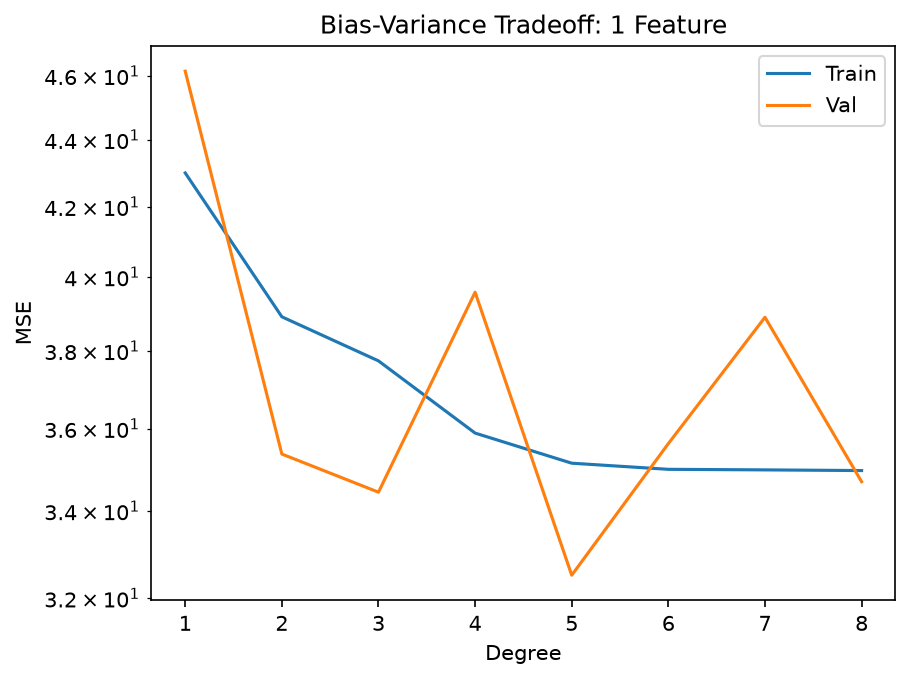
\includegraphics[width=0.8\textwidth]{outputs/e18_graph.png}
\end{center}
\vspace{\baselineskip}

\noindent \textbf{Result:}\\
Program executed successfully.

\end{document}

